\documentclass{article}
\usepackage[utf8]{inputenc}
\usepackage{graphicx}
\usepackage[spanish]{babel}
\usepackage{float}
%%%%%%%%%%%%%%%%%%%%%%%%%%%%%%%
\title{Reporte de la Actividad 5}
\author{Rolando A. Fimbres G.}
\date{6 de marzo de 2018}
%%%%%%%%%%%%%%%%%%%%%%%%%%%%%%%%%%%5
\begin{document}
\maketitle
\section{Introdución}
La práctica nos muestra un script cuya meta es generar un archivo con extensión \textbf{csv}. Dentro de éste script, podemos ver que se han utilizado, los datos mensuales del sondeo de nuestra estación elegida. Mediante algunos comandos de Emacs como lo son \textit{cat} y \textit{egrep} la ejecución del script provocaría la limitación de los datos a los señalados. Éstos son: Showalter, LIFT, CAPE, Temp, PW, thick; entre otros.\\
El objetivo de la práctica es modificar el script para solo obtener los datos de: CAPE y PW. Ejecutar el script modificado para después limpiarlo con las herramientas de Emacs; de manera que, el archivo csv muestre únicamente los datos con el siguiente formato:\\
\begin{center}
12Z  01  01  2017,  0.00,  9.42\\
\end{center}
Trás haber finalizado la limpieza del csv, el archivo está listo para ser analizado. Desde la terminal utilizamos algunos comandos de Emacs para separar el archivo en dos. Uno que tenga los datos de 00Z y otro con los de 12Z. Ahora abriremos un jupyter notebook desde la terminal. Dentro seguiremos la guía del análisis propocionada por el profesor en un hipervínculo en la página de pbworks.\\
\section{Descripción de Conceptos Físicos}
Ahora continuaré describiendo las variables analizadas: CAPE y PW.\\
Las siglas CAPE vienen del inglés Convective Available Potential Energy (Energía Potencial Convectiva Disponible) y es la cantidad de energía que una parcela de aire tendría si se levantara una cierta distancia vertical a través de la atmósfera.\\
El CAPE es efectivamente la flotabilidad positiva de una parcela de aire y un indicador de inestabilidad atmosférica, el cual resulta ser muy valioso para predecir un tiempo severo (fenómenos meteorológicos peligrosos).\\
El CAPE existe en la condicional e inestable capa de la tropósfera, la free convective layer (capa de convección libre), FLC, por sus siglas en inglés, donde una parcela de aire ascendente es más caliente que el aire en el ambiente. Éste se mide en joules por kilogramo de aire, además es calculado al integrar verticalmente la flotabilidad local de una parcela del level of free convection (nivel de convección libre), LFC, al equilibrium level (nivel de equilibrio), EL.\\
\begin{center}
$CAPE=\int_{z_{f}}^{z_{n}}(\frac{T_{v,parcel}-T_{v,env}}{T_{v,env}})dz$
\end{center}
Las siglas PW provinen del inglés y significan Precipitable Water (Agua Precipitable) y ésta representa la profundidad de agua en una columna de la atmósfera, si toda el agua en esa columna fuera precipitada como lluvia. Usualmente ésta es medida en milímetros (mm) o pulgadas (in).\\
Existen varias técnicas de medición. Uno tipo de medición es el basado en las medidas de irradiancia solar en dos longitudes de onda, una en la banda de absorción de agua y la otra no. La columna de agua precipitable es determinada utilizando las irradiancias de ambas bandas y la Ley de Beer-Lambert.\\
Por definición, la transmitancia de una muestra de material está relacionado a su profundidad óptica $\tau$ y su absorbancia $A$ como\\
\begin{center}
$T=\frac{\Phi_e^t}{\Phi_e^i}=e^{-\tau}=10^{-A}$
\end{center}
donde\\
\begin{itemize}
\item $\Phi_e^t$ es el flujo radiante transmitido por la muestra del material.
\item $\Phi_e^i$ es el flujo radiante recibido por la la muestra del material.\\
\end{itemize}
\section{Limpieza y Preparación de Datos}
Como se mencionaba anteriormente en la introdución se realizó una limpieza de datos para prepararlos para ser analizados. Ésto fué posible gracias a las herramientas de Emacs. Iniciamos poniendo un marcador al inicio de la palabra que necesitabamos eliminar. Después seleccionamos la palabra/frase/espacio que deseábamos reemplazar. Posteriormente hicimos uso del comando Wipe (Ctrl + W) para mandar lo seleccionado a la memoria. Luego el comando Yank (Ctrl + Y) para vaciar lo seleccionado de nuevo a su lugar. Después nos posicionamos en el inicio del archivo presionando 'Esc + <'.\\
A partir de éste momento podemos iniciar el proceso de reemplazo de la frase. Presionamos 'Esc + \%' y vemos en la pequeña ventana inferior una frace que nos indica cuál es la frase que queremos reemplazar. Utilizamos el comando Yank pues la frase a reemplazar sigue guardada en la memoria. Luego leemos que nos pide escribir la frase por la cual queremos reemplazar lo guardado en la memoria. En éste caso si lo que queremos reemplazar es una oración sin dato importante alguno solo presionamos un espacio y enter. Veremos que se seleccionarán todas aquellas frases iguales a las especificadas, procedemos a presionar '!' para de una sola ver realizar todos los reemplazos necesarios.\\
Ya que hemos hecho ésto hay una ultima cosa a realizar antes de analizar los archivos. Ésto es separar los archivos segun las horas: 00Z y 12Z. para ésto accedemos a la carpeta de nuestra actividad desde la terminal y escribimos lo siguiente:\\
\begin{figure}[H]
	\centering
    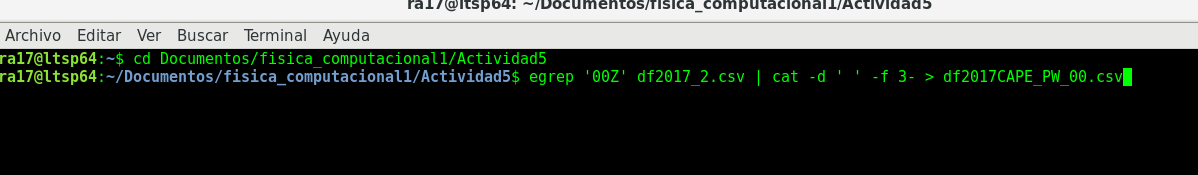
\includegraphics[width=\linewidth]{r5.png}\\
\end{figure}
De ésta manera repetimos para '12Z' y tendremos dos archivos para analizar por separado.\\
\section{Análisis de Datos}
El análisis por medio de pandas se llevará acabo en un entorno jupyter. Abrimos un jupyter notebook desde la terminal estándo previamente en la carpeta de la actividad. Ahora realizaremos cuatro gráficos por cada uno de los archivos a analizar. El primer gráfico será uno de data frame head que mostrará los primeros cinco datos de CAPE y PW según la fecha correspondiente. El segundo es un gráfico de cajas de CAPE contra meses. El tercero es un joint plot de PW contra CAPE. La última es de un modelo lineal de PW contra CAPE utilizando colores para cada mes.\\
\section{Resultados del Análisis}
\begin{figure}[H]
	\centering
    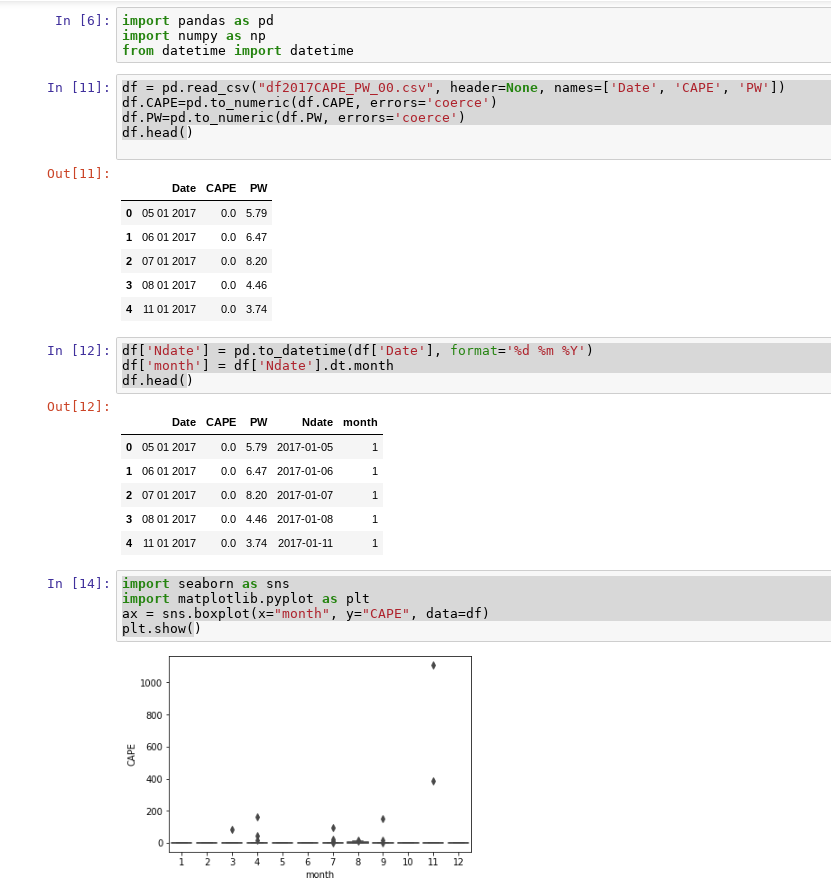
\includegraphics[width=\linewidth]{p1.png}
\end{figure}
\begin{figure}[H]
	\centering
    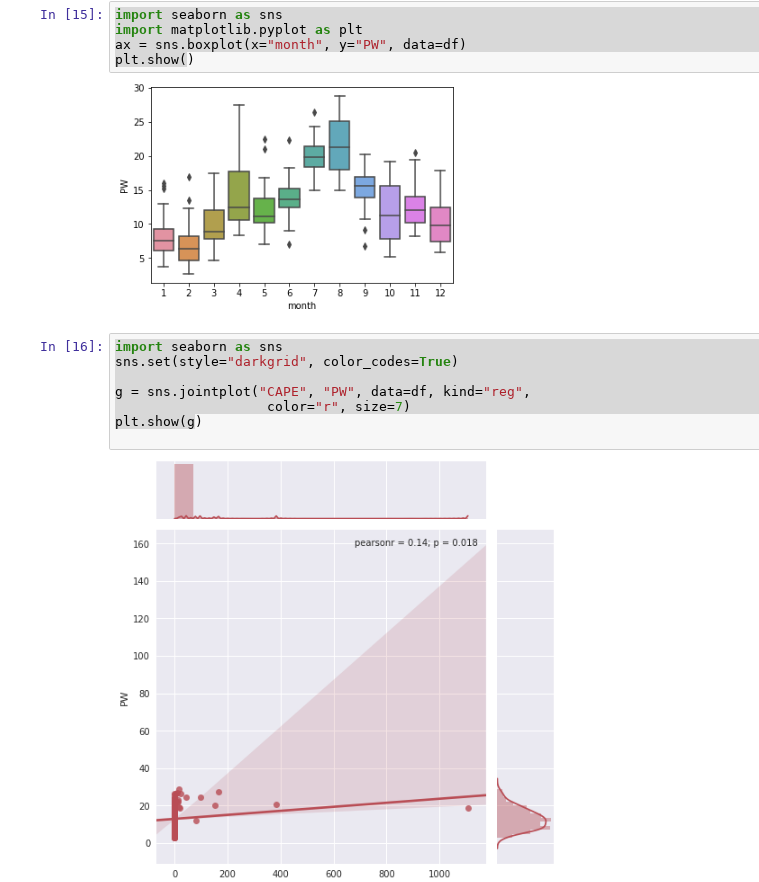
\includegraphics[width=\linewidth]{p2.png}
\end{figure}
\begin{figure}[H]
	\centering
    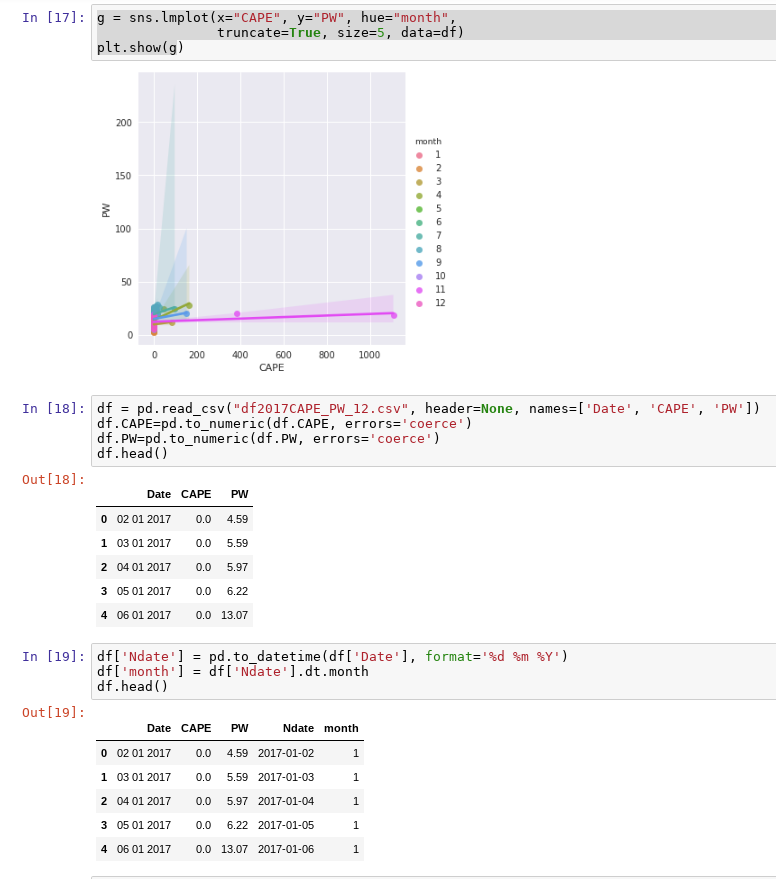
\includegraphics[width=\linewidth]{p3.png}
\end{figure}
\begin{figure}[H]
	\centering
    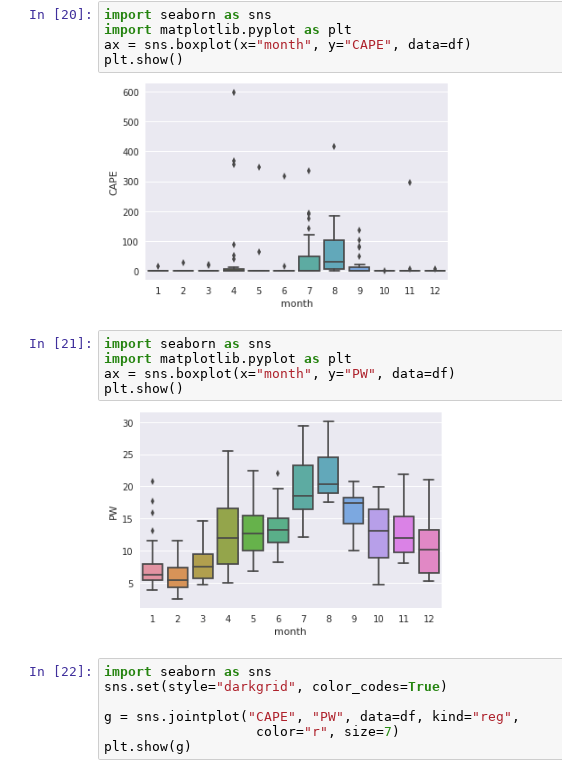
\includegraphics[width=\linewidth]{p4.png}
\end{figure}
\begin{figure}[H]
	\centering
    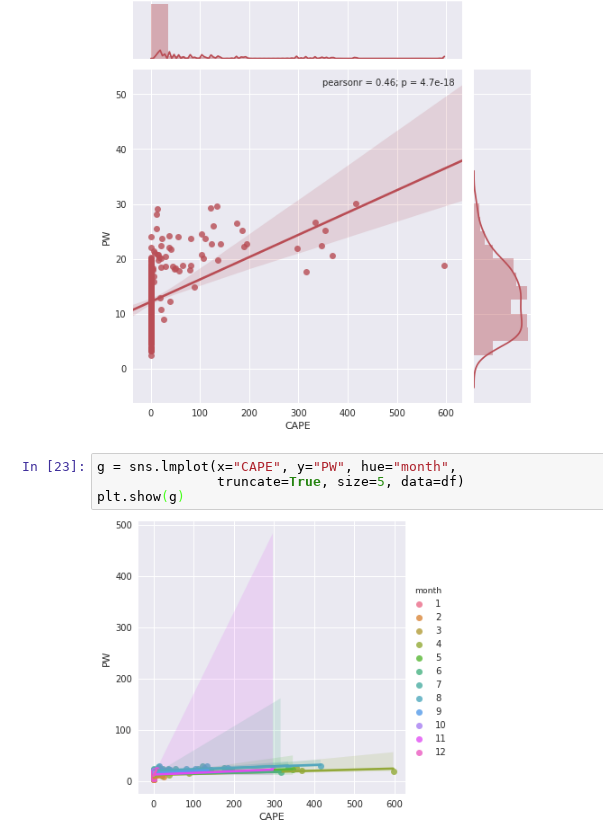
\includegraphics[width=\linewidth]{p5.png}
\end{figure}
\section{Apéndice}
1. ¿Cómo se te hizo ésta actividad? ¿Compleja, difícil, sencilla?\\
Me pareció sencilla.\\
2. ¿Qué te llamó más la atención?\\
El uso se los comandos de Emacs para limpiar el archivo.\\
3. ¿Qué parte fue la que menos te interesó hacer?\\
El reporte.\\
4. ¿Cómo mejorarías ésta actividad? ¿Qué le faltó? ¿Qué sobró?\\
Me parece bien así como está.\\
5. ¿Hasta éste punto, que te parece el uso de Jupyter para programar en Python?\\
Me parece bien porque solo necesitas una conexión a internet para poder programar donde sea.\\
\section{Conclusiones}
Las habilidades aprendidas en ésta práctica las considero muy útiles pues estoy completamente seguro que haré uso de ellas no solo mientras lleve la materia sino durante mucho tiempo. Me ha dado una nueva perspectiva acerca del tratamiento previo al análisis de datos. Cosa que considero muy importante para mantenerlos con una buena estructura.\\
\section{Bibliografía}
\begin{itemize}
\item M. W. Moncrieff, M.J. Miller (1976). \textit{The dynamics and simulation of tropical cumulonimbus and squall lines}.
\item Shu, Frank (1992). \textit{The Physics of Astrophysics, volume II: Gas dynamics}. 
\item  Hsu, S.A.; Blanchard, B.W. (15 October 1989). \textit{The Relationship Between Total Precipitable Water and Surface-Level Humidity Over the Sea Surface: A Further Evaluation}.
\item https://es.sharelatex.com/learn
\end{itemize}
\end{document}
